%%%%%%%%%%%%%%%%%%%%%%%%%%%%%%%%%%%%%%%%%%%%%%%%%%%%%%%%%%%%%%%%%%%%%%%%%%%%%%%%%%
\begin{frame}[fragile]\frametitle{}
\begin{center}
{\Large Data Science}
\end{center}
\end{frame}

%%%%%%%%%%%%%%%%%%%%%%%%%%%%%%%%%%%%%%%%%%%%%%%%%%%%%%%%%%%%%%%%%%%%%%%%%%%%%%%%%%
\begin{frame}[fragile]\frametitle{Graph Data Science (GDS)}
\begin{itemize}
\item GDS is delivered as library and a plugin to the Neo4j Graph Database. 
\item GDS comes in both a free Community and paid Enterprise license; differences in regard to performance and enterprise capabilities. 
\item However, all analytics functionality, including graph algorithms and machine learning methods, are the same between both licenses.
\end{itemize}

\end{frame}

%%%%%%%%%%%%%%%%%%%%%%%%%%%%%%%%%%%%%%%%%%%%%%%%%%%%%%%%%%%%%%%%%%%%%%%%%%%%%%%%%%
\begin{frame}\frametitle{  What are the big questions  graph data science helps answer?  }

\begin{center}
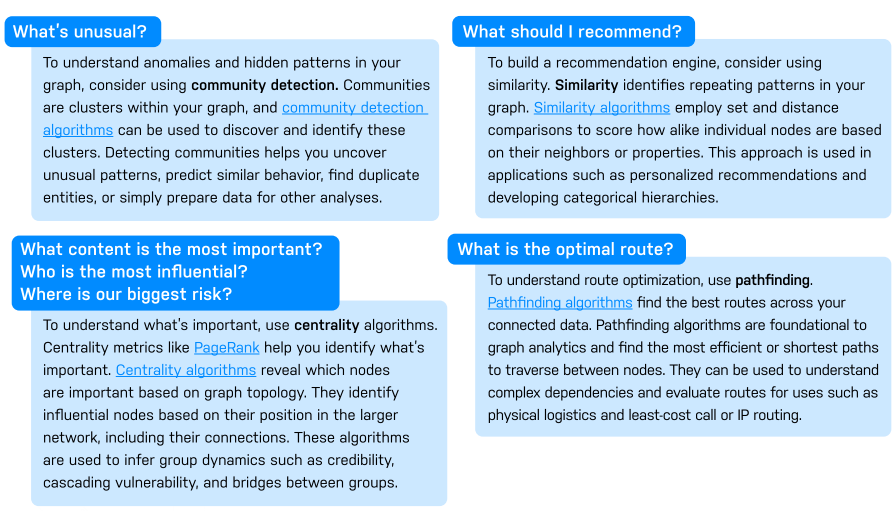
\includegraphics[width=\linewidth,keepaspectratio]{neo4j104}
\end{center}	  


{\tiny (Ref: 5 Graph Data Science Basics Everyone Should Know - neo4j)}
\end{frame}


%%%%%%%%%%%%%%%%%%%%%%%%%%%%%%%%%%%%%%%%%%%%%%%%%%%%%%%%%%%%%%%%%%%%%%%%%%%%%%%%%%
\begin{frame}[fragile]\frametitle{Installation}

\begin{itemize}
\item Once you install and open Neo4j Desktop, you will find GDS in the Plugins tab of a database
\item The installer will download the GDS library and install it in the plugins/ directory of the database. 
\end{itemize}

\begin{center}
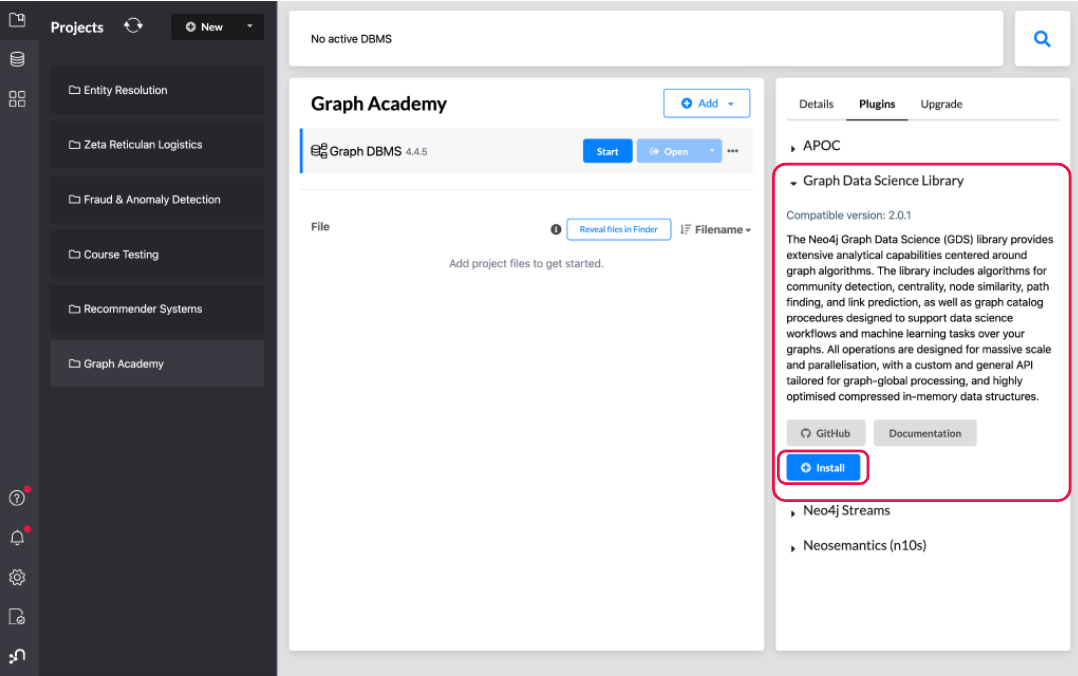
\includegraphics[width=0.7\linewidth,keepaspectratio]{neo4j93}
\end{center}	

{\tiny (Ref: Introduction to Neo4j Graph Data Science - neo4j)}
\end{frame}

%%%%%%%%%%%%%%%%%%%%%%%%%%%%%%%%%%%%%%%%%%%%%%%%%%%%%%%%%%%%%%%%%%%%%%%%%%%%%%%%%%
\begin{frame}[fragile]\frametitle{How GDS Works}

\begin{itemize}
\item At a high-level, GDS works by transforming and loading data into an in-memory format that is optimized for high-performance graph analytics. 
\item GDS provides graph algorithms, feature engineering, and machine learning methods to execute on this in-memory graph format.
\item Workflow: 
	\begin{itemize}
	\item Read data from the Neo4j database, transform it, and load it into an in-memory graph (aka  projecting a graph and refer to the in-memory graph as a graph projection). Collection of graph projections is called as Graph Catalog
	\item Execute Algorithms
	\item Store Results
	\end{itemize}
\end{itemize}

\begin{center}
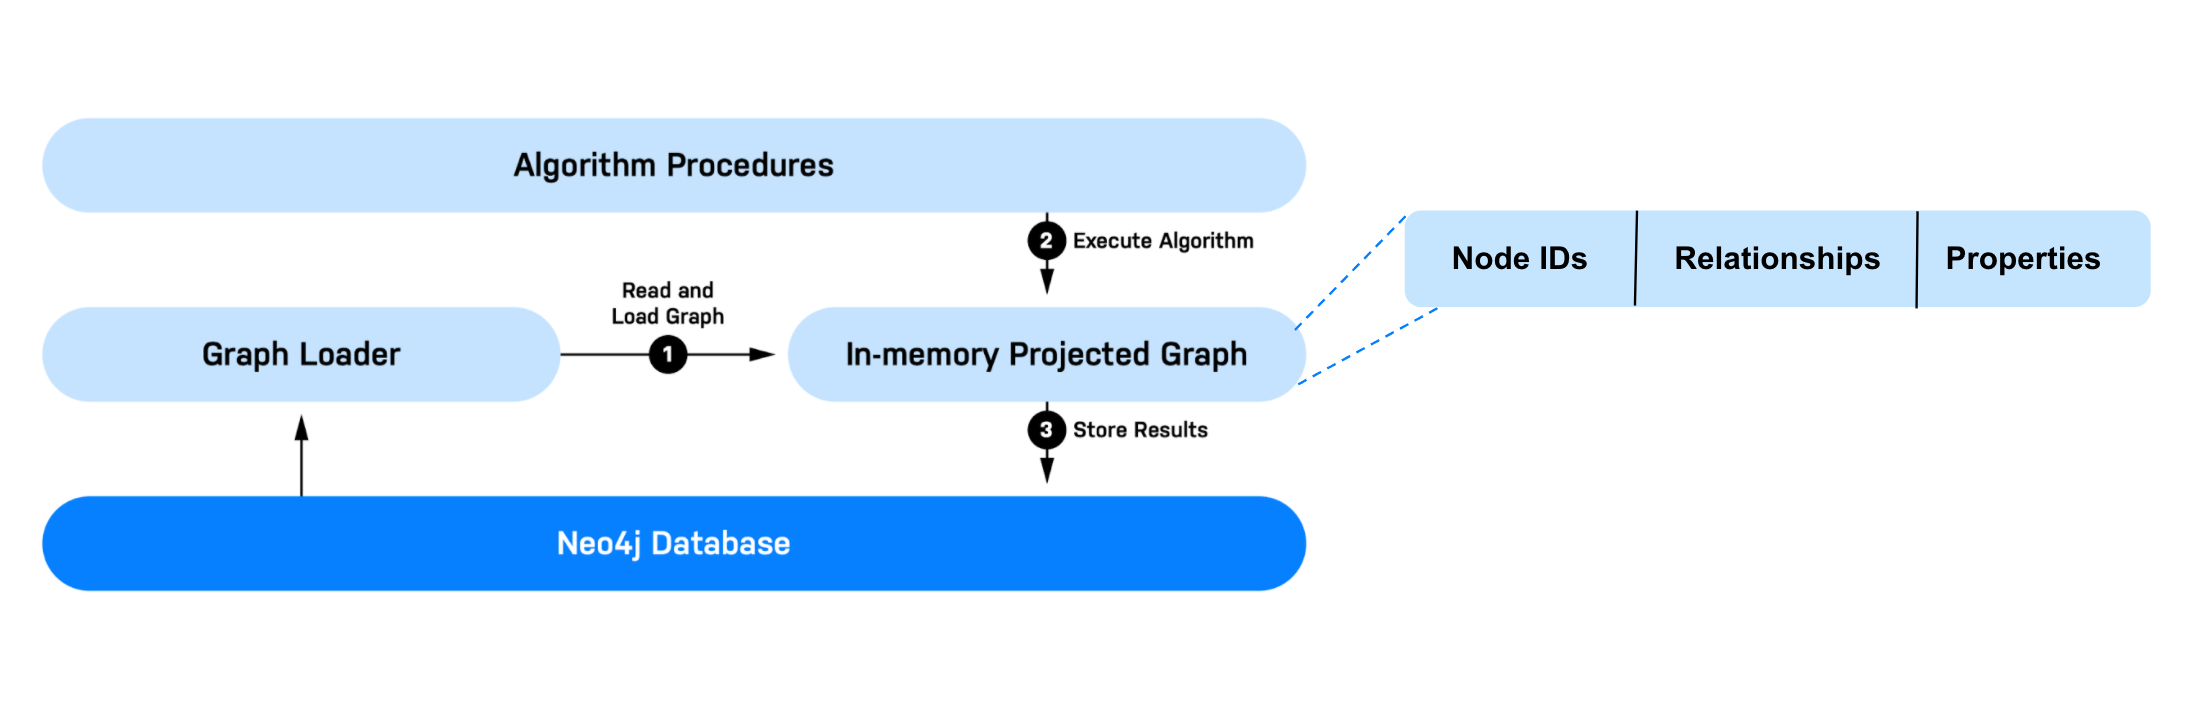
\includegraphics[width=0.8\linewidth,keepaspectratio]{neo4j94}
\end{center}	

{\tiny (Ref: Introduction to Neo4j Graph Data Science - neo4j)}
\end{frame}

%%%%%%%%%%%%%%%%%%%%%%%%%%%%%%%%%%%%%%%%%%%%%%%%%%%%%%%%%%%%%%%%%%%%%%%%%%%%%%%%%%
\begin{frame}[fragile]\frametitle{GDS Configuration}
\begin{columns}
\begin{column}{0.5\textwidth}

\begin{itemize}
\item GDS runs greedily in respect to system resources which means it will use as much memory and CPU cores as it needs - not exceeding limits configured by the user.
\item GDS uses multiple CPU cores for graph projections, algorithms, and writing results. This allows GDS to parallelize its computations and significantly speed up processing time.
\item GDS runs within a Neo4j instance and is therefore subject to the general Neo4j memory configuration. 
\end{itemize}

\end{column}
\begin{column}{0.5\textwidth}  %%<--- here

\begin{center}
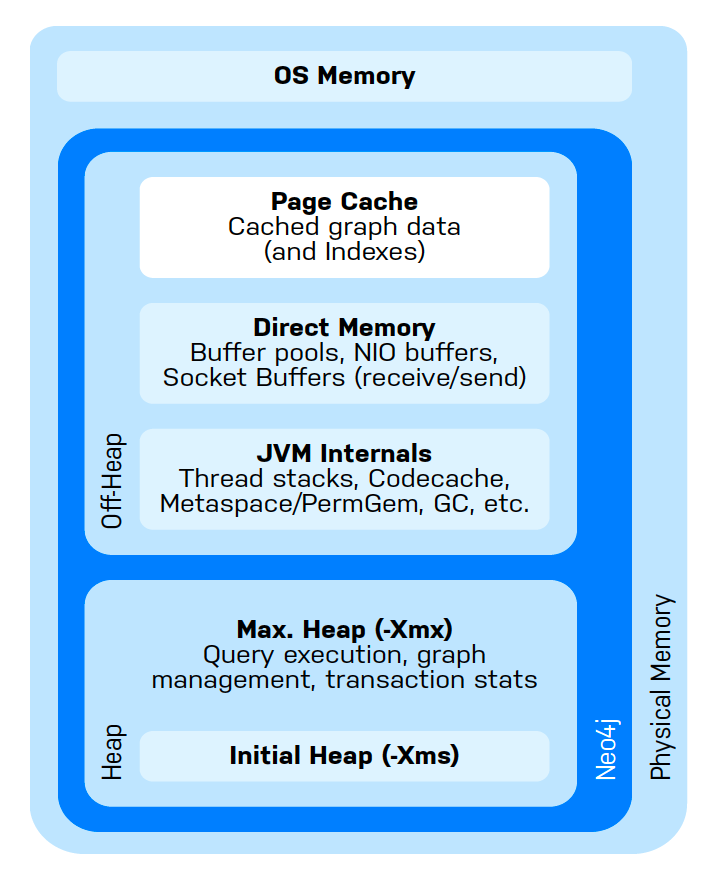
\includegraphics[width=0.8\linewidth,keepaspectratio]{neo4j95}
\end{center}	

{\tiny (Ref: Introduction to Neo4j Graph Data Science - neo4j)}
\end{column}
\end{columns}
\end{frame}

%%%%%%%%%%%%%%%%%%%%%%%%%%%%%%%%%%%%%%%%%%%%%%%%%%%%%%%%%%%%%%%%%%%%%%%%%%%%%%%%%%
\begin{frame}[fragile]\frametitle{Graph Catalog}

\begin{itemize}
\item You can call graph catalog operations with commands of the form \lstinline|CALL gds.graph.<command>|
\item For example, we can list the graph projections that currently exist in our database with  \lstinline|CALL gds.graph.list()|
\item In the recommendations graph, we can create a projection from the Actor and Movie nodes and the ACTED\_IN relationship with \lstinline|CALL gds.graph.project('my-graph-projection', ['Actor','Movie'], 'ACTED_IN')|
\item Now list graphs again we should see information on the graph we just made \lstinline|CALL gds.graph.list() YIELD graphName, nodeCount, relationshipCount, schema|
\end{itemize}

\begin{center}
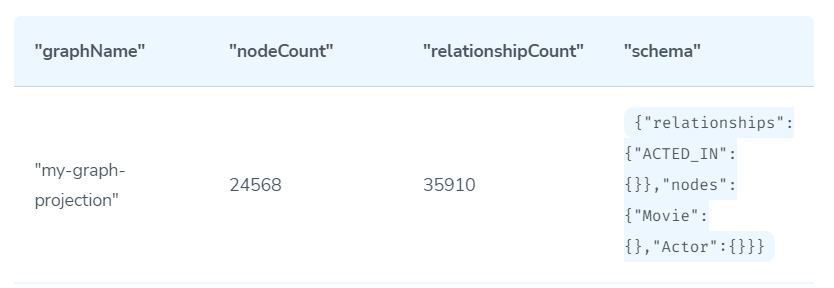
\includegraphics[width=0.8\linewidth,keepaspectratio]{neo4j96}
\end{center}	

{\tiny (Ref: Introduction to Neo4j Graph Data Science - neo4j)}
\end{frame}

%%%%%%%%%%%%%%%%%%%%%%%%%%%%%%%%%%%%%%%%%%%%%%%%%%%%%%%%%%%%%%%%%%%%%%%%%%%%%%%%%%
\begin{frame}[fragile]\frametitle{Running Algorithms}

\begin{itemize}
\item Say, run degree centrality on Actor nodes. 
\item \lstinline|CALL gds.degree.mutate('my-graph-projection', {mutateProperty:'numberOfMoviesActedIn'})|
\item This will count the number of movies each actor was in and store it on a node property called numberOfMoviesActedIn inside the projection (it will not be written back to the database yet).
\end{itemize}

\begin{lstlisting}
CALL gds.graph.streamNodeProperty('my-graph-projection','numberOfMoviesActedIn')
YIELD nodeId, propertyValue
RETURN gds.util.asNode(nodeId).name AS actorName, propertyValue AS numberOfMoviesActedIn
ORDER BY numberOfMoviesActedIn DESCENDING, actorName LIMIT 10| 
\end{lstlisting}

\end{frame}

%%%%%%%%%%%%%%%%%%%%%%%%%%%%%%%%%%%%%%%%%%%%%%%%%%%%%%%%%%%%%%%%%%%%%%%%%%%%%%%%%%
\begin{frame}[fragile]\frametitle{Running Algorithms}

\begin{itemize}
\item The graph catalog has two methods for export:
\begin{itemize}
\item gds.graph.export to export a graph into a new database - effectively copying the projection into a separate Neo4j database
\item 
gds.beta.graph.export.csv to export a graph to csv files
\end{itemize}

\item  To write the property back to the database we could use the writeNodeProperties operation: \lstinline|CALL gds.graph.writeNodeProperties('my-graph-projection',['numberOfMoviesActedIn'], ['Actor'])|
\item To take the results from our algorithm calculations and stream them into another process:
\end{itemize}


\end{frame}


%%%%%%%%%%%%%%%%%%%%%%%%%%%%%%%%%%%%%%%%%%%%%%%%%%%%%%%%%%%%%%%%%%%%%%%%%%%%%%%%%%
\begin{frame}[fragile]\frametitle{Projects}

There are 2 primary types of projections in GDS, native projections and cypher projections.

\begin{itemize}
\item Native projections are optimized for efficiency and performance to support graph data science at scale.
\item Cypher projections are optimized for flexibility and customization to support exploratory analysis, experimentation, and smaller graph projections.
\item If you attempt to create a new graph projection with a name that already exists, you will receive an error. To continue you will first have to run the gds.graph.drop() procedure to drop the existing graph projection.
\item '*' can be used to include all nodes and/or relationships in the database.
\end{itemize}

\end{frame}


%%%%%%%%%%%%%%%%%%%%%%%%%%%%%%%%%%%%%%%%%%%%%%%%%%%%%%%%%%%%%%%%%%%%%%%%%%%%%%%%%%
\begin{frame}[fragile]\frametitle{Projects}

There are 2 primary types of projections in GDS, native projections and cypher projections.

\begin{itemize}

\item  When you call \lstinline|gds.graph.project()| you are using a native projection. 
\item Native projections provide the best performance by reading from the Neo4j store files directly
\item Additional features:
	\begin{itemize}
	\item the inclusion of numeric node and relationship properties
	\item altering relationship direction or "orientation"
		\begin{itemize}
			\item NATURAL: same direction as in the database (default)
			\item REVERSE: opposite direction as in the database
			\item UNDIRECTED: undirected
			\end{itemize}

	\item aggregating parallel relationships
	\end{itemize}
\end{itemize}

\end{frame}


%%%%%%%%%%%%%%%%%%%%%%%%%%%%%%%%%%%%%%%%%%%%%%%%%%%%%%%%%%%%%%%%%%%%%%%%%%%%%%%%%%
\begin{frame}[fragile]\frametitle{Including Node and Relationship Properties}

\begin{itemize}
\item Node and relationship properties may be useful to consider in graph analytics. 
\item They can be used as weights in graph algorithms and features for machine learning.
\item Below is an example of including multiple movie node properties and the rating relationship property.
\end{itemize}

\begin{lstlisting}
CALL gds.graph.drop('native-proj', false);

CALL gds.graph.project(
    'native-proj',
    ['User', 'Movie'],
    {RATED: {orientation: 'UNDIRECTED'}},
    {
        nodeProperties:{
            revenue: {defaultValue: 0}, // (1)
            budget: {defaultValue: 0},
            runtime: {defaultValue: 0}
        },
        relationshipProperties: ['rating'] // (3)
    }
);
\end{lstlisting}

\end{frame}

%%%%%%%%%%%%%%%%%%%%%%%%%%%%%%%%%%%%%%%%%%%%%%%%%%%%%%%%%%%%%%%%%%%%%%%%%%%%%%%%%%
\begin{frame}[fragile]\frametitle{Parallel Relationship}

\begin{itemize}
\item The Neo4j database allows you to store multiple relationships of the same type and direction between two nodes.
\item These are colloquially known as parallel relationships. 
\item For example, consider a graph of financial transaction data where users send money to one another. If a user sends money to the same user multiple times this can form multiple parallel relationships.
\end{itemize}

\begin{center}
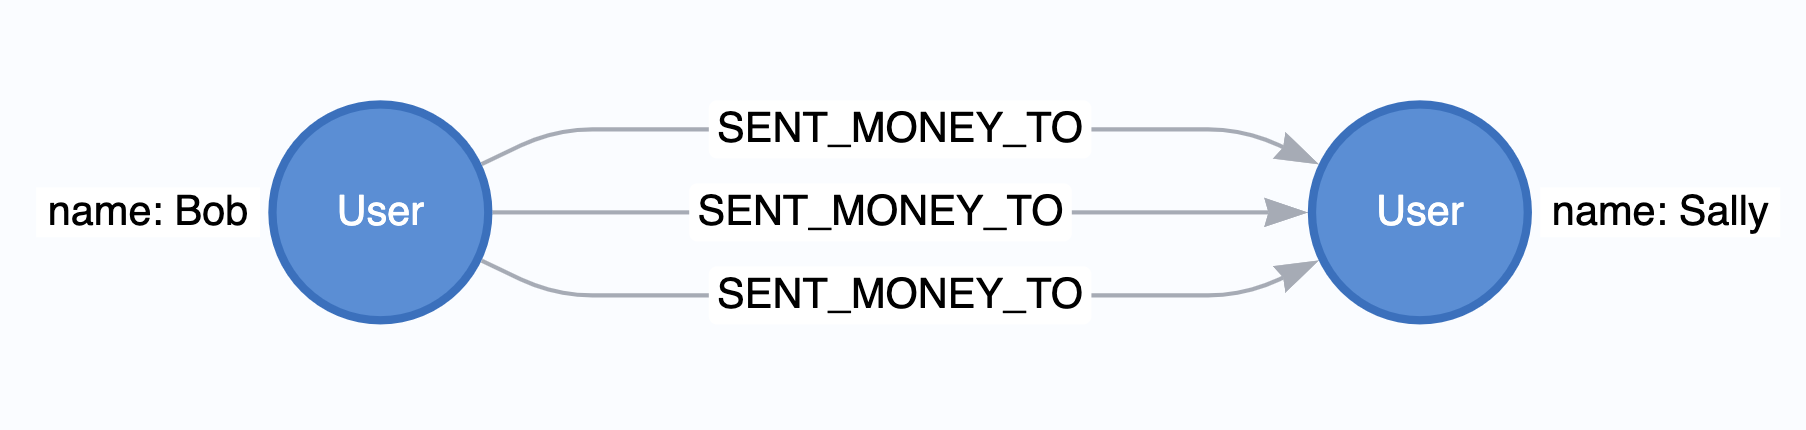
\includegraphics[width=0.8\linewidth,keepaspectratio]{neo4j97}
\end{center}	

{\tiny (Ref: Introduction to Neo4j Graph Data Science - neo4j)}
\end{frame}

%%%%%%%%%%%%%%%%%%%%%%%%%%%%%%%%%%%%%%%%%%%%%%%%%%%%%%%%%%%%%%%%%%%%%%%%%%%%%%%%%%
\begin{frame}[fragile]\frametitle{Parallel Relationship Aggregation}

\begin{itemize}
\item Sometimes you will want to aggregate these parallel relationships into a single relationship in preparation for running graph algorithms or machine learning. 
\item This is because graph algorithms may count each relationship between two nodes separately when all we need to consider is whether a single relationship exists between them. 
\item Other times we may want to weight the connection between two nodes higher if more parallel relationships exists, but it’s not always easy to do so without aggregating the relationships first depending on which algorithm you use.
\end{itemize}

\begin{center}
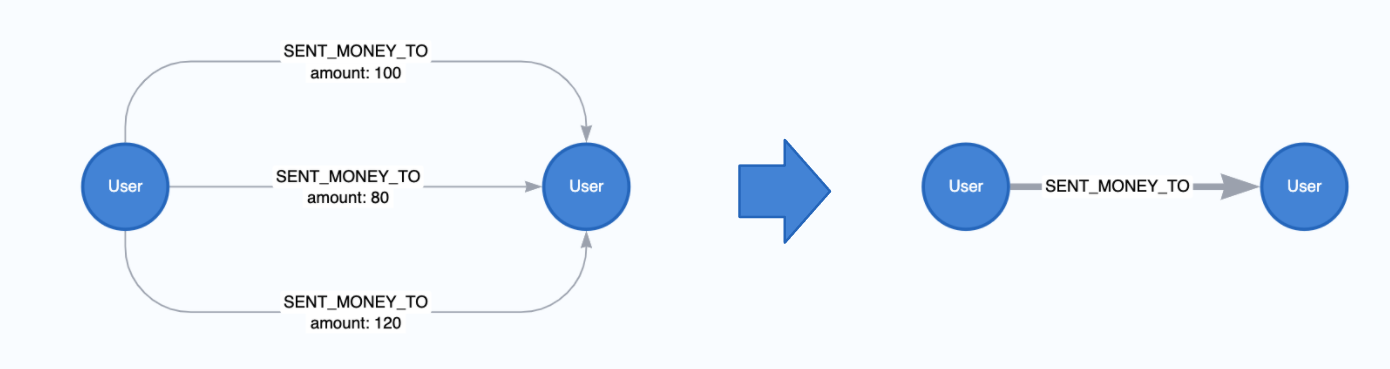
\includegraphics[width=0.8\linewidth,keepaspectratio]{neo4j98}
\end{center}	

{\tiny (Ref: Introduction to Neo4j Graph Data Science - neo4j)}

\end{frame}

%%%%%%%%%%%%%%%%%%%%%%%%%%%%%%%%%%%%%%%%%%%%%%%%%%%%%%%%%%%%%%%%%%%%%%%%%%%%%%%%%%
\begin{frame}[fragile]\frametitle{Parallel Relationship Aggregation}

\begin{center}
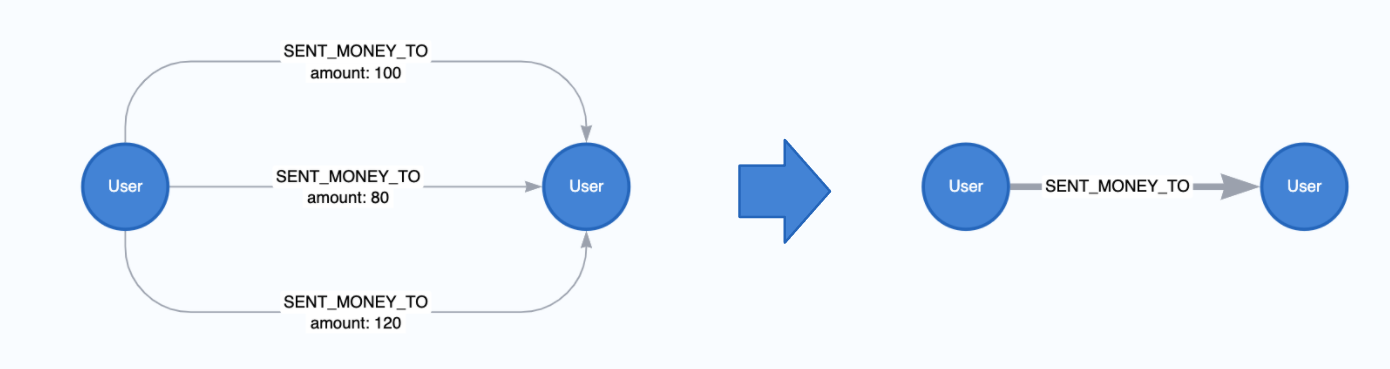
\includegraphics[width=0.8\linewidth,keepaspectratio]{neo4j98}
\end{center}	

{\tiny (Ref: Introduction to Neo4j Graph Data Science - neo4j)}

\begin{lstlisting}
CALL gds.graph.project(
  'user-proj',
  ['User'],
  {
    SENT_MONEY_TO: { aggregation: 'SINGLE' }
  }
);
\end{lstlisting}
\end{frame}

%%%%%%%%%%%%%%%%%%%%%%%%%%%%%%%%%%%%%%%%%%%%%%%%%%%%%%%%%%%%%%%%%%%%%%%%%%%%%%%%%%
\begin{frame}[fragile]\frametitle{Parallel Relationship Aggregation}

We can create a property with the count of the relationships as well - like so:

\begin{center}
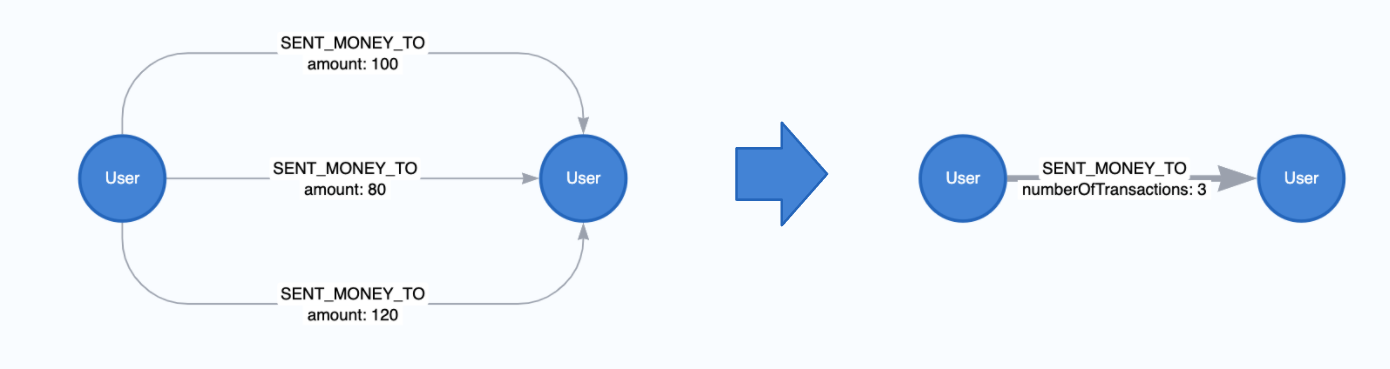
\includegraphics[width=0.8\linewidth,keepaspectratio]{neo4j99}
\end{center}	

\begin{lstlisting}
CALL gds.graph.project(
  'user-proj',
  ['User'],
  {
    SENT_MONEY_TO: {
      properties: {
        numberOfTransactions: {
          // the wildcard '*' is a placeholder, signaling that
          // the value of the relationship property is derived
          // and not based on Neo4j property.
          property: '*',
          aggregation: 'COUNT'
        }
      }
    }
  }
);
\end{lstlisting}
\end{frame}

%%%%%%%%%%%%%%%%%%%%%%%%%%%%%%%%%%%%%%%%%%%%%%%%%%%%%%%%%%%%%%%%%%%%%%%%%%%%%%%%%%
\begin{frame}[fragile]\frametitle{Cypher Projections}

\begin{itemize}
\item While the native projection is scalable and fast, its filtering and aggregation capabilities aren’t as flexible as Cypher. \item The Cypher projection, as its name implies, uses Cypher to define the projection pattern, and as such, enables more flexibility.
\item Cypher projections are intended to be used in exploratory analysis and developmental phases where additional flexibility and/or customization is needed.
\item Cypher Projections have a diminished focus on performance relative to native projections and as a result won’t perform as quickly or as well on larger graphs.
\item A Cypher projection takes three mandatory arguments: graphName, nodeQuery, and relationshipQuery. 
\end{itemize}


\end{frame}

%%%%%%%%%%%%%%%%%%%%%%%%%%%%%%%%%%%%%%%%%%%%%%%%%%%%%%%%%%%%%%%%%%%%%%%%%%%%%%%%%%
\begin{frame}[fragile]\frametitle{Cypher Projections}

\begin{lstlisting}
CALL gds.graph.project.cypher(
  'proj-cypher',
  'MATCH (a:Actor) RETURN id(a) AS id, labels(a) AS labels',
  'MATCH (a1:Actor)-[:ACTED_IN]->(m:Movie)<-[:ACTED_IN]-(a2)
   WHERE m.year >= 1990 AND m.revenue >= 1000000
   RETURN id(a1) AS source , id(a2) AS target, count(*) AS actedWithCount, "ACTED_WITH" AS type'
);
\end{lstlisting}

\end{frame}

%%%%%%%%%%%%%%%%%%%%%%%%%%%%%%%%%%%%%%%%%%%%%%%%%%%%%%%%%%%%%%%%%%%%%%%%%%%%%%%%%%
\begin{frame}[fragile]\frametitle{Applying Algorithms}

\begin{itemize}
\item Apply degree centrality , except we will weight the degree centrality by actedWithCount property and also directly stream the top 10 results back. 
\item This counts how many times the actor has acted with other actors in recent, high grossing movies.
\item The graph is not set up to answer this question well with a direct native projection. However, we can use a cypher projection to filter to the appropriate nodes and perform an aggregation to create an ACTED\_WITH relationship that has a actedWithCount property going directly between actor nodes.
\end{itemize}

\begin{lstlisting}
CALL gds.degree.stream('proj-cypher',{relationshipWeightProperty: 'actedWithCount'})
YIELD nodeId, score
RETURN gds.util.asNode(nodeId).name AS name, score
ORDER BY score DESC LIMIT 10

name						score
Robert De Niro 	123.0
Bruce Willis 		120.0
:
\end{lstlisting}

\end{frame}

%%%%%%%%%%%%%%%%%%%%%%%%%%%%%%%%%%%%%%%%%%%%%%%%%%%%%%%%%%%%%%%%%%%%%%%%%%%%%%%%%%
\begin{frame}[fragile]\frametitle{Usages}

Some things which are prevented in Native Projection are possible in Cypher Projection.
 
\begin{itemize}
\item Complex Filtering: Using node and/or relationship property conditions or other more complex MATCH/WHERE conditions to filter the graph, rather than just node label and relationship types.
\item Aggregating Multi-Hop Paths with Weights: The relationship projection required aggregating the \lstinline|(Actor)-[ACTED_IN]-(Movie)-[ACTED_IN]-(Actor)| pattern to a \lstinline|(Actor)-[ACTED_WITH {actedWithCount}]-(Actor)| pattern where the actedWithCount is a relationship weight property. This type of projection, where we need to transform multi-hop paths into an aggregated relationship that connects the source and target node, is a commonly occurring pattern in graph analytics.
\end{itemize}


\end{frame}


%%%%%%%%%%%%%%%%%%%%%%%%%%%%%%%%%%%%%%%%%%%%%%%%%%%%%%%%%%%%%%%%%%%%%%%%%%%%%%%%%%
\begin{frame}[fragile]\frametitle{Execution Modes}

GDS algorithms are classified into:


\begin{itemize}
\item Production-quality: Indicates that the algorithm has been tested in regard to stability and scalability. \lstinline|gds.<algorithm>|
\item Beta: Indicates that the algorithm is a candidate for the production-quality tier. \lstinline|gds.beta.<algorithm>|
\item Alpha: Indicates that the algorithm is experimental and might be changed or removed at any time. \lstinline|gds.alpha.<algorithm>|
\end{itemize}

\end{frame}

%%%%%%%%%%%%%%%%%%%%%%%%%%%%%%%%%%%%%%%%%%%%%%%%%%%%%%%%%%%%%%%%%%%%%%%%%%%%%%%%%%
\begin{frame}[fragile]\frametitle{Execution Modes}

\begin{itemize}
\item GDS algorithms have following Execution modes and they determine how the results of the algorithm are handled.
	\begin{itemize}
	\item stream: Returns the result of the algorithm as a stream of records.
	\item stats: Returns a single record of summary statistics, but does not write to the Neo4j database or modify any data.
	\item mutate: Writes the results of the algorithm to the in-memory graph projection and returns a single record of summary statistics.
	\item write: Writes the results of the algorithm back the Neo4j database and returns a single record of summary statistics.
	\end{itemize}
\item Only production tier algorithms guarantee the existence of all execution modes.
\item GDS offers an estimation procedure which allows you to estimate the memory needed for using an algorithm on your data BEFORE actually executing it. Just append \lstinline|.estimate| to the command
\end{itemize}


Overall syntax:

\begin{lstlisting}
CALL gds[.<tier>].<algorithm>.<execution-mode>[.<estimate>](
	graphName: STRING,
	configuration: MAP
)
\end{lstlisting}

\end{frame}


%%%%%%%%%%%%%%%%%%%%%%%%%%%%%%%%%%%%%%%%%%%%%%%%%%%%%%%%%%%%%%%%%%%%%%%%%%%%%%%%%%
\begin{frame}[fragile]\frametitle{Algorithms}
Graph data science brings together:
\begin{itemize}
\item Graph statistics, queries, and visualization drive exploration and insights. 
\item Graph analytics builds on graph statistics by answering specific questions and gaining 
insights from connections in existing or historical data
\item Graph-enhanced ML is the application of graph data and analytics results to train ML models 
or support probabilistic decisions within an AI system.
\end{itemize}

\begin{center}
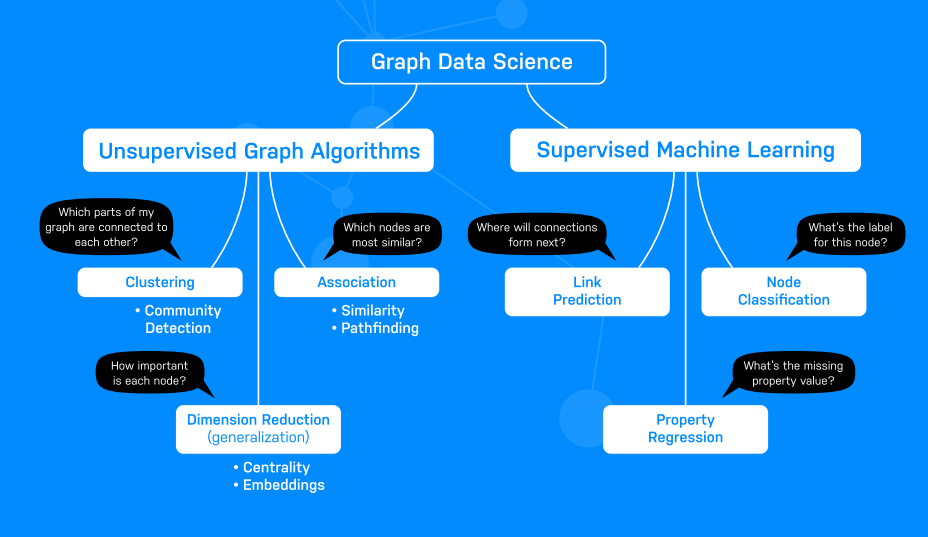
\includegraphics[width=0.8\linewidth,keepaspectratio]{neo4j102}
\end{center}	

{\tiny (Ref: 5 Graph Data Science Basics Everyone Should Know  - neo4j)}
\end{frame}



%%%%%%%%%%%%%%%%%%%%%%%%%%%%%%%%%%%%%%%%%%%%%%%%%%%%%%%%%%%%%%%%%%%%%%%%%%%%%%%%%%
\begin{frame}[fragile]\frametitle{Centrality Algorithms}

 Centrality algorithms are used to determine the importance of distinct nodes in a graph. Applications are:
 
\begin{itemize}
\item Recommendations: Identify and recommend the most influential or popular items in your content or product offering catalog
\item Supply chain analytics: find the most critical node in your supply chain, whether it be a supplier in a network, a raw material that is part of a manufactured product, or a port in a route
\item Fraud \& Anomaly Detection: Find users with many shared identifiers or who otherwise act as a bridge between many communities
\end{itemize}


\end{frame}

%%%%%%%%%%%%%%%%%%%%%%%%%%%%%%%%%%%%%%%%%%%%%%%%%%%%%%%%%%%%%%%%%%%%%%%%%%%%%%%%%%
\begin{frame}[fragile]\frametitle{Degree Centrality}


\begin{itemize}
\item counts the number of relationships a node has.
\item specifically calculate out-degree centrality which is the count of outgoing relationships from a node.
\item Below is an example of using degree centrality to count the number of movies each actor has acted in. 
\item Then stream the degree centrality.First create the graph projection.
\item The top three actors should be "Robert De Niro", "Bruce Willis", and "Nicolas Cage."
\end{itemize}

\begin{lstlisting}
CALL gds.graph.project('proj', ['Actor','Movie'], 'ACTED_IN');

//get top 5 most prolific actors (those in the most movies)
//using degree centrality which counts number of `ACTED_IN` relationships
CALL gds.degree.stream('proj')
YIELD nodeId, score
RETURN gds.util.asNode(nodeId).name AS actorName, score AS numberOfMoviesActedIn
ORDER BY numberOfMoviesActedIn DESCENDING, actorName LIMIT 5
\end{lstlisting}

\end{frame}

%%%%%%%%%%%%%%%%%%%%%%%%%%%%%%%%%%%%%%%%%%%%%%%%%%%%%%%%%%%%%%%%%%%%%%%%%%%%%%%%%%
\begin{frame}[fragile]\frametitle{PageRank}


\begin{itemize}
\item  for measuring the influence of nodes in a directed graph, particularly where the relationships imply some form of flow of movement such as in payment networks, supply chain and logistics, communications, routing, and graphs of website and links.
\item estimates the importance of a node by counting the number of incoming relationships from neighboring nodes weighted by the importance as well as out-degree centrality of those neighbors
\item The underlying assumption is that more important nodes are likely to have proportionately more incoming relationships from other important nodes.
\item First, create the graph projection. We can use a Cypher projection in this case to obtain a graph where we have \lstinline|(Person)-[:DIRECTED_ACTOR]->(Person)|. this graph can be traversed to understand the influence across directors and actors.
\item Next stream PageRank to find the top 5 most influential people in director-actor network.
\end{itemize}


\end{frame}

%%%%%%%%%%%%%%%%%%%%%%%%%%%%%%%%%%%%%%%%%%%%%%%%%%%%%%%%%%%%%%%%%%%%%%%%%%%%%%%%%%
\begin{frame}[fragile]\frametitle{PageRank}


\begin{lstlisting}
//drop last graph projection
CALL gds.graph.drop('proj', false);

//create Cypher projection for network of people directing actors
//filter to recent high grossing movies
CALL gds.graph.project.cypher(
  'proj',
  'MATCH (a:Person) RETURN id(a) AS id, labels(a) AS labels',
  'MATCH (a1:Person)-[:DIRECTED]->(m:Movie)<-[:ACTED_IN]-(a2)
   WHERE m.year >= 1990 AND m.revenue >= 10000000
   RETURN id(a1) AS source , id(a2) AS target, count(*) AS actedWithCount,
    "DIRECTED_ACTOR" AS type'
);

CALL gds.pageRank.stream('proj')
YIELD nodeId, score
RETURN gds.util.asNode(nodeId).name AS personName, score AS influence
ORDER BY influence DESCENDING, personName LIMIT 5

\end{lstlisting}

\end{frame}

%%%%%%%%%%%%%%%%%%%%%%%%%%%%%%%%%%%%%%%%%%%%%%%%%%%%%%%%%%%%%%%%%%%%%%%%%%%%%%%%%%
\begin{frame}[fragile]\frametitle{Other Centrality Algorithms}

 
\begin{itemize}
\item Betweenness Centrality: Measures the extent to which a node stands between the other nodes in a graph. It is often used to find nodes that serve as a bridge from one part of a graph to another.
\item Eigenvector Centrality: Measures the transitive influence of nodes. Similar to PageRank, but works only on the largest eigenvector of the adjacency matrix so does not converge in the same way and tends to more strongly favor high degree nodes. It can be more appropriate in certain use cases, particularly those with undirected relationships.
\item Article Rank: A variant of PageRank which assumes that relationships originating from low-degree nodes have a higher influence than relationships from high-degree nodes.
\end{itemize}


\end{frame}



%%%%%%%%%%%%%%%%%%%%%%%%%%%%%%%%%%%%%%%%%%%%%%%%%%%%%%%%%%%%%%%%%%%%%%%%%%%%%%%%%%
\begin{frame}[fragile]\frametitle{Path Finding Algorithms}

 To find the shortest path between two or more nodes or evaluate the availability and quality of paths. Applications:
 
\begin{itemize}
\item  Supply chain analytics: Identifying the fastest path between an origin and a destination or between a raw material and a finished product
\item  Customer Journey: Analyzing the events that make up a customer’s experience. In healthcare for example, this can be the experience of an in-patient from admission to discharge.
\end{itemize}

A common, industry standard, path finding algorithm is Dijkstra. It computes the shortest path between a source and a target node, e.g. shortest path between the actors "Kevin Bacon" and "Denzel Washington". This should give you a 4 hop path between Kevin Bacon and Denzel Washington.

\end{frame}


%%%%%%%%%%%%%%%%%%%%%%%%%%%%%%%%%%%%%%%%%%%%%%%%%%%%%%%%%%%%%%%%%%%%%%%%%%%%%%%%%%
\begin{frame}[fragile]\frametitle{Path Finding Algorithms}

\begin{lstlisting}
CALL gds.graph.project('proj',
    ['Person','Movie'],
    {
        ACTED_IN:{orientation:'UNDIRECTED'},
        DIRECTED:{orientation:'UNDIRECTED'}
    }
);

MATCH (a:Actor)
WHERE a.name IN ['Kevin Bacon', 'Denzel Washington']
WITH collect(id(a)) AS nodeIds
CALL gds.shortestPath.dijkstra.stream('proj', {sourceNode:nodeIds[0], TargetNode:nodeIds[1]})
YIELD sourceNode, targetNode, path
RETURN gds.util.asNode(sourceNode).name AS sourceNodeName,
    gds.util.asNode(targetNode).name AS targetNodeName,
    nodes(path) as path;
\end{lstlisting}


\end{frame}

%%%%%%%%%%%%%%%%%%%%%%%%%%%%%%%%%%%%%%%%%%%%%%%%%%%%%%%%%%%%%%%%%%%%%%%%%%%%%%%%%%
\begin{frame}[fragile]\frametitle{Other Path Finding Algorithms}

 Shortest path between two nodes:
\begin{itemize}
\item A* Shortest Path: An extension of Dijkstra that uses a heuristic function to speed up computation.
\item Yen’s Algorithm Shortest Path: An extension of Dijkstra that allows you to find multiple, the top k, shortest paths.
\end{itemize}

Shortest path between a source node and multiple other target nodes:

\begin{itemize}
\item Dijkstra Single-Source Shortest Path: Dijkstra implementation for shortest path between one source and multiple targets.
\item Delta-Stepping Single-Source Shortest Path: Parallelized shortest path computation. Computes faster than Dijkstra single-source shortest Path but uses more memory.
\end{itemize}

General path search between a source node and multiple other target nodes:
\begin{itemize}

\item Breadth First Search: Searches paths in order of increasing distance from the source node on each iteration.
\item Depth First Search: Searches as far as possible along a single multi-hop path on each iteration.
\end{itemize}
\end{frame}


%%%%%%%%%%%%%%%%%%%%%%%%%%%%%%%%%%%%%%%%%%%%%%%%%%%%%%%%%%%%%%%%%%%%%%%%%%%%%%%%%%
\begin{frame}[fragile]\frametitle{Community Detection Algorithms}

 
 \begin{itemize}
\item to evaluate how groups of nodes may be clustered or partitioned in the graph
\item distinguishing and assigning ids to these node groups for downstream analytics, visualization, or other processing.
\item Applications:
	\begin{itemize}
	\item Fraud detection: Finding fraud rings by identifying accounts that have frequent suspicious transactions and/or share identifiers between one another.
	\item Customer 360: Disambiguating multiple records and interactions into a single customer profile so an organization has an aggregated source of truth for each customer.
	\item Market segmentation: dividing a target market into approachable subgroups based on priorities, behaviors, interests, and other criteria.
	\end{itemize}
\end{itemize}



\end{frame}

%%%%%%%%%%%%%%%%%%%%%%%%%%%%%%%%%%%%%%%%%%%%%%%%%%%%%%%%%%%%%%%%%%%%%%%%%%%%%%%%%%
\begin{frame}[fragile]\frametitle{Louvain Community Detection}

 
 \begin{itemize}
\item maximizes a modularity score for each community with a hierarchical clustering approach that recursively merges communities together. 
\item means evaluating how much more densely connected the nodes within a community are, compared to how connected they would be in a random network.
\item Being a stochastic algorithm, the community assignments may change a bit when re-run. When the graph does not have a naturally well-defined community structure the changes between runs can become more significant. \lstinline|seedProperty| is used to  assign initial community ids and help with consistency between runs. 
\item Create graph and run algorithm, then we can verify the communityId node properties in the projection with a stream operation.
\end{itemize}


\end{frame}

%%%%%%%%%%%%%%%%%%%%%%%%%%%%%%%%%%%%%%%%%%%%%%%%%%%%%%%%%%%%%%%%%%%%%%%%%%%%%%%%%%
\begin{frame}[fragile]\frametitle{Louvain Community Detection}

\begin{lstlisting}
CALL gds.graph.project('proj', ['Movie', 'Person'], {
    ACTED_IN:{orientation:'UNDIRECTED'},
    DIRECTED:{orientation:'UNDIRECTED'}
});

CALL gds.louvain.mutate('proj', {mutateProperty:'communityId'})

CALL gds.graph.streamNodeProperty('proj','communityId', ['Person'])
YIELD nodeId, propertyValue
WITH gds.util.asNode(nodeId) AS n, propertyValue AS communityId
WHERE n:Person
RETURN n.name, communityId LIMIT 10
\end{lstlisting}

\end{frame}

%%%%%%%%%%%%%%%%%%%%%%%%%%%%%%%%%%%%%%%%%%%%%%%%%%%%%%%%%%%%%%%%%%%%%%%%%%%%%%%%%%
\begin{frame}[fragile]\frametitle{Other Community Detection}

 
 \begin{itemize}
\item Label Propagation: Similar intent as Louvain. Fast algorithm that parallelizes well. Great for large graphs.
\item Weakly Connected Components (WCC): Partitions the graph into sets of connected nodes such that
\item Every node is reachable from any other node in the same set
\item No path exists between nodes from different sets
\item Triangle Count: Counts the number of triangles for each node. Can be used to detect the cohesiveness of communities and stability of the graph.
\item Local Clustering Coefficient: Computes the local clustering coefficient for each node in the graph which is an indicator for how the node clusters with its neighbors.
\end{itemize}

\end{frame}

%%%%%%%%%%%%%%%%%%%%%%%%%%%%%%%%%%%%%%%%%%%%%%%%%%%%%%%%%%%%%%%%%%%%%%%%%%%%%%%%%%
\begin{frame}[fragile]\frametitle{Node Embeddings}

\begin{itemize}
\item to compute low-dimensional vector representations of nodes such that similarity between vectors (eg. dot product) approximates similarity between nodes in the original graph
\item Node embedding vectors don’t offer insights by themselves, they are created to enable Machine/Deep Learning
\item Applications
	\begin{itemize}
	\item Exploratory Data Analysis (EDA) such as visualizing the embeddings in a TSNE plot to better understand the graph structure and potential clusters of nodes
	\item Similarity Measurements: Node embedding allows you to scale similarity inferences in large graphs using K Nearest Neighbor (KNN) or other techniques.
	\item Features for Machine Learning: Node embedding vectors naturally plug in as features for a variety of machine learning problems. 
	\end{itemize}
\item GDS, apart from FastRP, has also implemented Node2Vec, which computes a vector representation of a node based on random walks in the graph, and GraphSage, which is an inductive modeling approach for computing node embeddings using node properties and graph structure.	
\end{itemize}

\end{frame}

%%%%%%%%%%%%%%%%%%%%%%%%%%%%%%%%%%%%%%%%%%%%%%%%%%%%%%%%%%%%%%%%%%%%%%%%%%%%%%%%%%
\begin{frame}[fragile]\frametitle{Node Embedding: FastRP}

\begin{itemize}
\item Fast Random Projection, or FastRP leverages probabilistic sampling techniques to generate sparse representations of the graph allowing for extremely fast calculation of embedding vectors that are comparative in quality to those produced with traditional random walk and neural net techniques such as Node2vec and GraphSage. 
\item Parameters
	\begin{itemize}
	\item embeddingDimension: length of the embedding vectors
	\item IterationWeights: This controls two aspects: the number of iterations for intermediate embeddings, and their relative impact on the final node embedding.
	\end{itemize}
\end{itemize}

\begin{lstlisting}
CALL gds.graph.project('proj', ['Movie', 'Person'], {
    ACTED_IN:{orientation:'UNDIRECTED'},
    DIRECTED:{orientation:'UNDIRECTED'}
});

CALL gds.fastRP.stream('proj',  {embeddingDimension:64, randomSeed:7474})
YIELD nodeId, embedding
WITH gds.util.asNode(nodeId) AS n, embedding
WHERE n:Person
RETURN id(n), n.name, embedding LIMIT 10
\end{lstlisting}

\end{frame}

%%%%%%%%%%%%%%%%%%%%%%%%%%%%%%%%%%%%%%%%%%%%%%%%%%%%%%%%%%%%%%%%%%%%%%%%%%%%%%%%%%
\begin{frame}[fragile]\frametitle{Similarity Algorithms}

 
\begin{itemize}
\item to infer similarity between pairs of nodes. 
\item run over the graph projection in bulk
\item When similar node pairs are identified according to the user specified metric and threshold, a relationship with a similarity score property is drawn between the pair.
\item Applications
	\begin{itemize}
	\item Fraud detection: finding potential fraud user accounts by analyzing how similar a set of new user accounts is to flagged accounts
	\item Recommendation Systems: In an online retail store, identifying items that pair to the one currently being viewed by a user to inform impressions and increase rate of purchase
	\item Entity Resolution: Identify nodes that are similar to one another based on activity or identifying information in the graph
	\end{itemize}
\item Algorithms 
	\begin{itemize}
	\item Node Similarity: Determines similarity between nodes based on the relative proportion of shared neighboring nodes in the graph. 
	\item K-Nearest Neighbor (KNN): Determines similarity based off node properties. The GDS KNN implementation can scale well for global inference over large graphs when tuned appropriately
	\end{itemize}	
\end{itemize}

\end{frame}

%%%%%%%%%%%%%%%%%%%%%%%%%%%%%%%%%%%%%%%%%%%%%%%%%%%%%%%%%%%%%%%%%%%%%%%%%%%%%%%%%%
\begin{frame}[fragile]\frametitle{Similarity Algorithms}

\begin{lstlisting}
CALL gds.graph.project('proj', ['Movie', 'Person'], {
    ACTED_IN:{orientation:'UNDIRECTED'},
    DIRECTED:{orientation:'UNDIRECTED'}
});

CALL gds.fastRP.mutate('proj',  {
    embeddingDimension:64,
    randomSeed:7474,
    mutateProperty:'embedding'
})

CALL gds.knn.stream('proj', {nodeLabels:['Person'], nodeProperties:['embedding'], topK:1})
YIELD  node1, node2, similarity
RETURN gds.util.asNode(node1).name AS actorName1,
    gds.util.asNode(node2).name AS actorName2,
    similarity
LIMIT 10
\end{lstlisting}
\end{frame}
%%%%%%%%%%%%%%%%%%%%%%%%%%%%%%%%%%%%%%%%%%%%%%%%%%%%%%%%%%%%%%%%%%%%%%%%%%%%%%%%%%
\begin{frame}[fragile]\frametitle{Machine Learning Overview}

 
\begin{itemize}
\item managed pipelines for end-to-end ML workflows. Data selection, feature engineering, data splitting, hyperparameter configuration, and training steps 
\item There are currently two supported types of ML pipelines:
	\begin{itemize}
	\item Node Classification Pipelines: Supervised binary and multi-class classification for nodes
	\item Link Prediction Pipelines: Supervised prediction for whether a relationship or "link" should exist between pairs of nodes
	\end{itemize}
\item Both pipelines have \lstinline|train| and \lstinline|predict| procedures.
\end{itemize}

\end{frame}

%%%%%%%%%%%%%%%%%%%%%%%%%%%%%%%%%%%%%%%%%%%%%%%%%%%%%%%%%%%%%%%%%%%%%%%%%%%%%%%%%%
\begin{frame}[fragile]\frametitle{Machine Learning: Classification}

Steps 1-6, the training steps, will be executed automatically by the pipeline. You will just be responsible for providing configuration and hyperparameters for them. 
 
\begin{center}
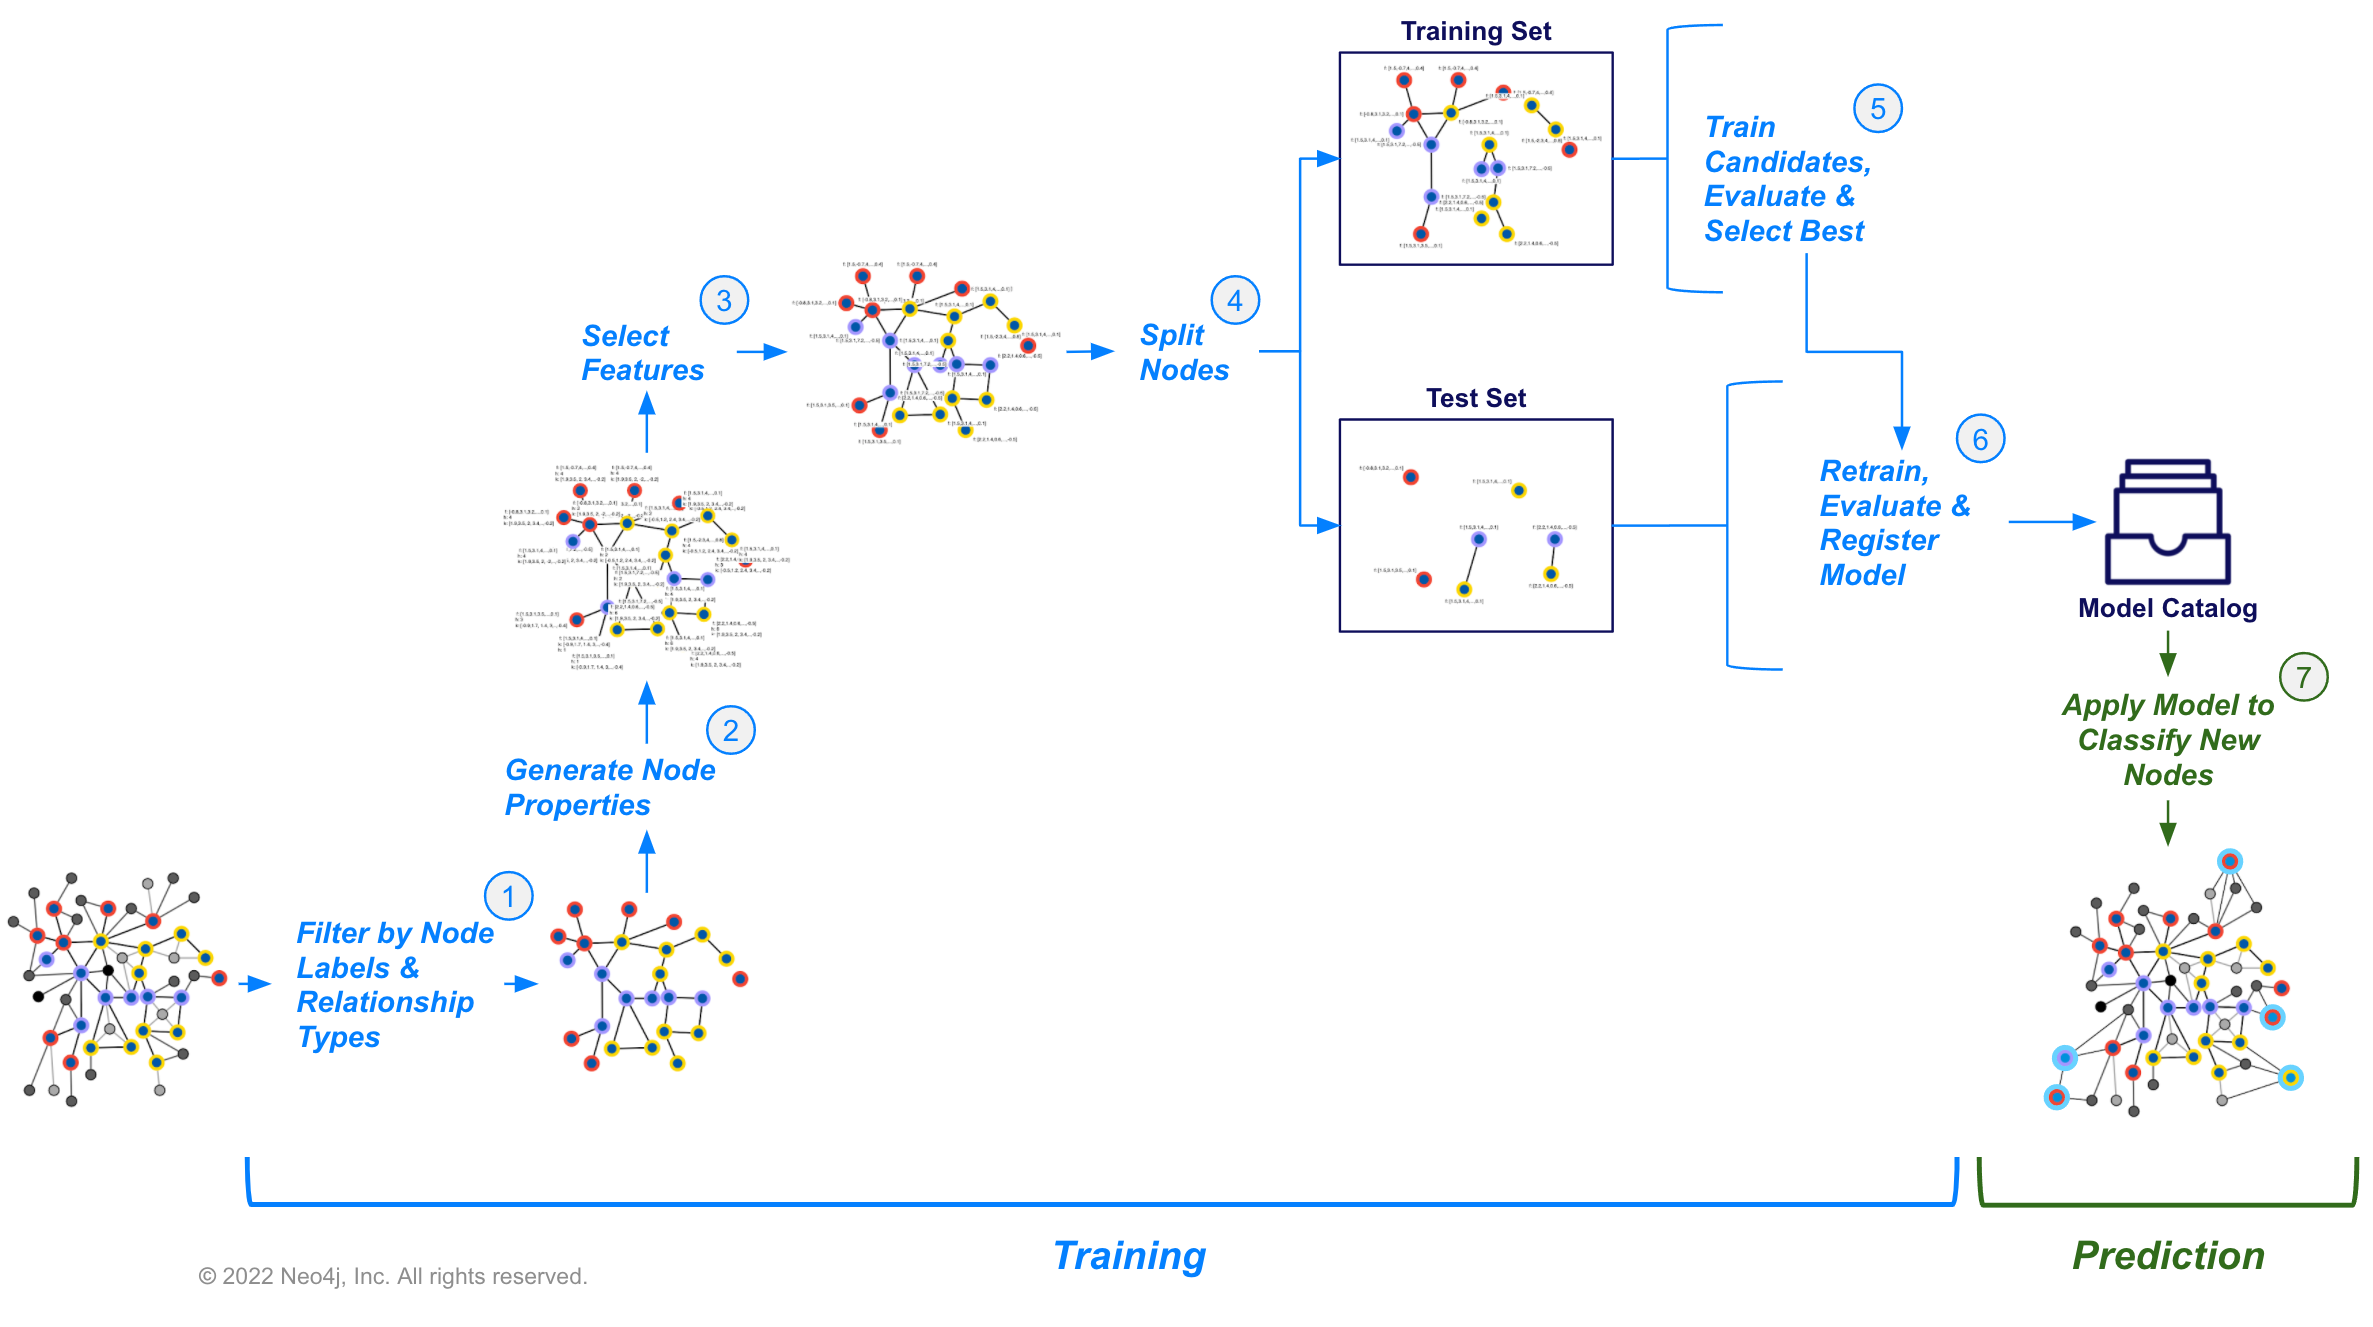
\includegraphics[width=\linewidth,keepaspectratio]{neo4j100}
\end{center}	


\end{frame}

%%%%%%%%%%%%%%%%%%%%%%%%%%%%%%%%%%%%%%%%%%%%%%%%%%%%%%%%%%%%%%%%%%%%%%%%%%%%%%%%%%
\begin{frame}[fragile]\frametitle{Machine Learning: Classification: Problem}

\begin{itemize}
\item Problem: to predict which movies in the graph are comedies which we will define as any movie that has a Genre of "Comedy".
\item Genre is currently represented by its own node in the graph. For this problem we need it represented as a property of the Movie node. 
\item For demonstration purposes we will assign a cls property which is 1 if the movie is a comedy and 0 otherwise.
\end{itemize}

\begin{lstlisting}
MATCH(m:Movie)-[:IN_GENRE]->(g)
WITH m , collect(g.name) AS genres
SET m.cls = toInteger('Comedy' IN genres)
RETURN count(m), m.cls;
\end{lstlisting}
\end{frame}

%%%%%%%%%%%%%%%%%%%%%%%%%%%%%%%%%%%%%%%%%%%%%%%%%%%%%%%%%%%%%%%%%%%%%%%%%%%%%%%%%%
\begin{frame}[fragile]\frametitle{Machine Learning: Classification: Preprocessing}

\begin{itemize}
\item The Movie node also has some missing property values for runtime and imdbRating, which could carry predictive signal for this problem.
\item We can either impute them or skip them. Lets skip.
\item While we do this we will filter the movies to only consider those released on or after 2010 as this type of data may drift overtime making data further in the past less relevant.
\end{itemize}

\begin{lstlisting}
MATCH(m:Movie)
WHERE m.year >= 2010
    AND m.runtime IS NOT NULL
    AND m.imdbRating IS NOT NULL
SET m:TrainMovie
RETURN count(m)
\end{lstlisting}
\end{frame}

%%%%%%%%%%%%%%%%%%%%%%%%%%%%%%%%%%%%%%%%%%%%%%%%%%%%%%%%%%%%%%%%%%%%%%%%%%%%%%%%%%
\begin{frame}[fragile]\frametitle{Machine Learning: Classification: Projection}

\begin{itemize}
\item Now we can project a graph using the TrainMovie node label. 
\item We will project mirroring natural and reverse relationships then use collapsePath to provide a monopartite projection which will make the graph easier to handle inside the pipeline for a quick demonstration.
\end{itemize}

\begin{lstlisting}
CALL gds.graph.project('proj',
    {
        Actor:{},
        TrainMovie:{ properties: ['cls', 'imdbRating', 'runtime']}
    },
    {
        ACTED_IN:{},
        HAD_ACTOR:{type:'ACTED_IN', orientation:'REVERSE'}
    }
);

CALL gds.alpha.collapsePath.mutate('proj',
  {
    relationshipTypes: ['HAD_ACTOR', 'ACTED_IN'],
    allowSelfLoops: false,
    mutateRelationshipType: 'SHARES_ACTOR_WITH'
  }
) YIELD relationshipsWritten;
\end{lstlisting}
\end{frame}

%%%%%%%%%%%%%%%%%%%%%%%%%%%%%%%%%%%%%%%%%%%%%%%%%%%%%%%%%%%%%%%%%%%%%%%%%%%%%%%%%%
\begin{frame}[fragile]\frametitle{Machine Learning: Classification: Configure the Pipeline}

\begin{itemize}
\item Create the Pipeline
\item Add Node Properties, generate FastRP embeddings
\item Select Node Properties as Features
\item Configure Node Splits
\item Add Model Candidates
\end{itemize}

\end{frame}

%%%%%%%%%%%%%%%%%%%%%%%%%%%%%%%%%%%%%%%%%%%%%%%%%%%%%%%%%%%%%%%%%%%%%%%%%%%%%%%%%%
\begin{frame}[fragile]\frametitle{Machine Learning: Classification: Configure the Pipeline}



\begin{lstlisting}
CALL gds.beta.pipeline.nodeClassification.create('pipe')

CALL gds.beta.pipeline.nodeClassification.addNodeProperty('pipe', 'fastRP', {
  embeddingDimension: 32,
  randomSeed: 7474,
  mutateProperty:'embedding'
})
YIELD name, nodePropertySteps;

// add degree centrality which will measure the number of other movies that share actors.
CALL gds.beta.pipeline.nodeClassification.addNodeProperty('pipe', 'degree', {
  mutateProperty:'degree'
})
YIELD name, nodePropertySteps;

// scale the runtime property
CALL gds.beta.pipeline.nodeClassification.addNodeProperty('pipe', 'alpha.scaleProperties', {
  nodeProperties: ['runtime'],
    scaler: 'Log',
  mutateProperty:'logRuntime'
})
YIELD name, nodePropertySteps;
\end{lstlisting}
\end{frame}
%%%%%%%%%%%%%%%%%%%%%%%%%%%%%%%%%%%%%%%%%%%%%%%%%%%%%%%%%%%%%%%%%%%%%%%%%%%%%%%%%%
\begin{frame}[fragile]\frametitle{Machine Learning: Classification: Configure the Pipeline}

\begin{lstlisting}
// configure the subset of node properties to use as features for the model
CALL gds.beta.pipeline.nodeClassification.selectFeatures(
    'pipe',
    ['imdbRating', 'logRuntime', 'embedding', 'degree'])
YIELD name, featureProperties;

// configure the data splitting
CALL gds.beta.pipeline.nodeClassification.configureSplit('pipe', {
 testFraction: 0.2,
  validationFolds: 5
})
YIELD splitConfig;

// creating model candidates with different parameters
CALL gds.beta.pipeline.nodeClassification.addLogisticRegression('pipe', {penalty: 0.0})
YIELD parameterSpace;
CALL gds.beta.pipeline.nodeClassification.addLogisticRegression('pipe', {penalty: 0.1})
YIELD parameterSpace;
CALL gds.beta.pipeline.nodeClassification.addLogisticRegression('pipe', {penalty: 1.0})
YIELD parameterSpace;
\end{lstlisting}
\end{frame}


%%%%%%%%%%%%%%%%%%%%%%%%%%%%%%%%%%%%%%%%%%%%%%%%%%%%%%%%%%%%%%%%%%%%%%%%%%%%%%%%%%
\begin{frame}[fragile]\frametitle{Machine Learning: Classification: Train the Pipeline}

\begin{itemize}
\item Apply node and relationship filters
\item Execute the above pipeline configuration steps
\item Train with cross-validation for all the candidate models
\item Select the best candidate according to the metric parameter. We will use ACCURACY for ease of interpretation
\item Retrain the winning model on the entire training set and perform a final evaluation on the test set according to the metric
\item Register the winning model in the model catalog

\end{itemize}

\end{frame}


%%%%%%%%%%%%%%%%%%%%%%%%%%%%%%%%%%%%%%%%%%%%%%%%%%%%%%%%%%%%%%%%%%%%%%%%%%%%%%%%%%
\begin{frame}[fragile]\frametitle{Machine Learning: Classification: Train the Pipeline}



\begin{lstlisting}
CALL gds.beta.pipeline.nodeClassification.train('proj', {
  pipeline: 'pipe',
  nodeLabels: ['TrainMovie'],
  modelName: 'nc-pipeline-model',
  targetProperty: 'cls',
  randomSeed: 7474,
  metrics: ['ACCURACY']
}) YIELD modelInfo
RETURN
  modelInfo.bestParameters AS winningModel,
  modelInfo.metrics.ACCURACY.train.avg AS avgTrainScore,
  modelInfo.metrics.ACCURACY.outerTrain AS outerTrainScore,
  modelInfo.metrics.ACCURACY.test AS testScore;
\end{lstlisting}
\end{frame}

%%%%%%%%%%%%%%%%%%%%%%%%%%%%%%%%%%%%%%%%%%%%%%%%%%%%%%%%%%%%%%%%%%%%%%%%%%%%%%%%%%
\begin{frame}[fragile]\frametitle{Machine Learning: Classification: Predict with the Pipeline}

\begin{lstlisting}
CALL gds.beta.pipeline.nodeClassification.predict.write(
  graphName: String,
  configuration: Map
)
YIELD
  preProcessingMillis: Integer,
  computeMillis: Integer,
  postProcessingMillis: Integer,
  writeMillis: Integer,
  nodePropertiesWritten: Integer,
  configuration: Map
\end{lstlisting}
	
\end{frame}



%%%%%%%%%%%%%%%%%%%%%%%%%%%%%%%%%%%%%%%%%%%%%%%%%%%%%%%%%%%%%%%%%%%%%%%%%%%%%%%%%%
\begin{frame}[fragile]\frametitle{Machine Learning: Link Prediction}

A binary classifier where the target is a 0-1 indicator, 0 for no link, 1 for a link.

\begin{center}
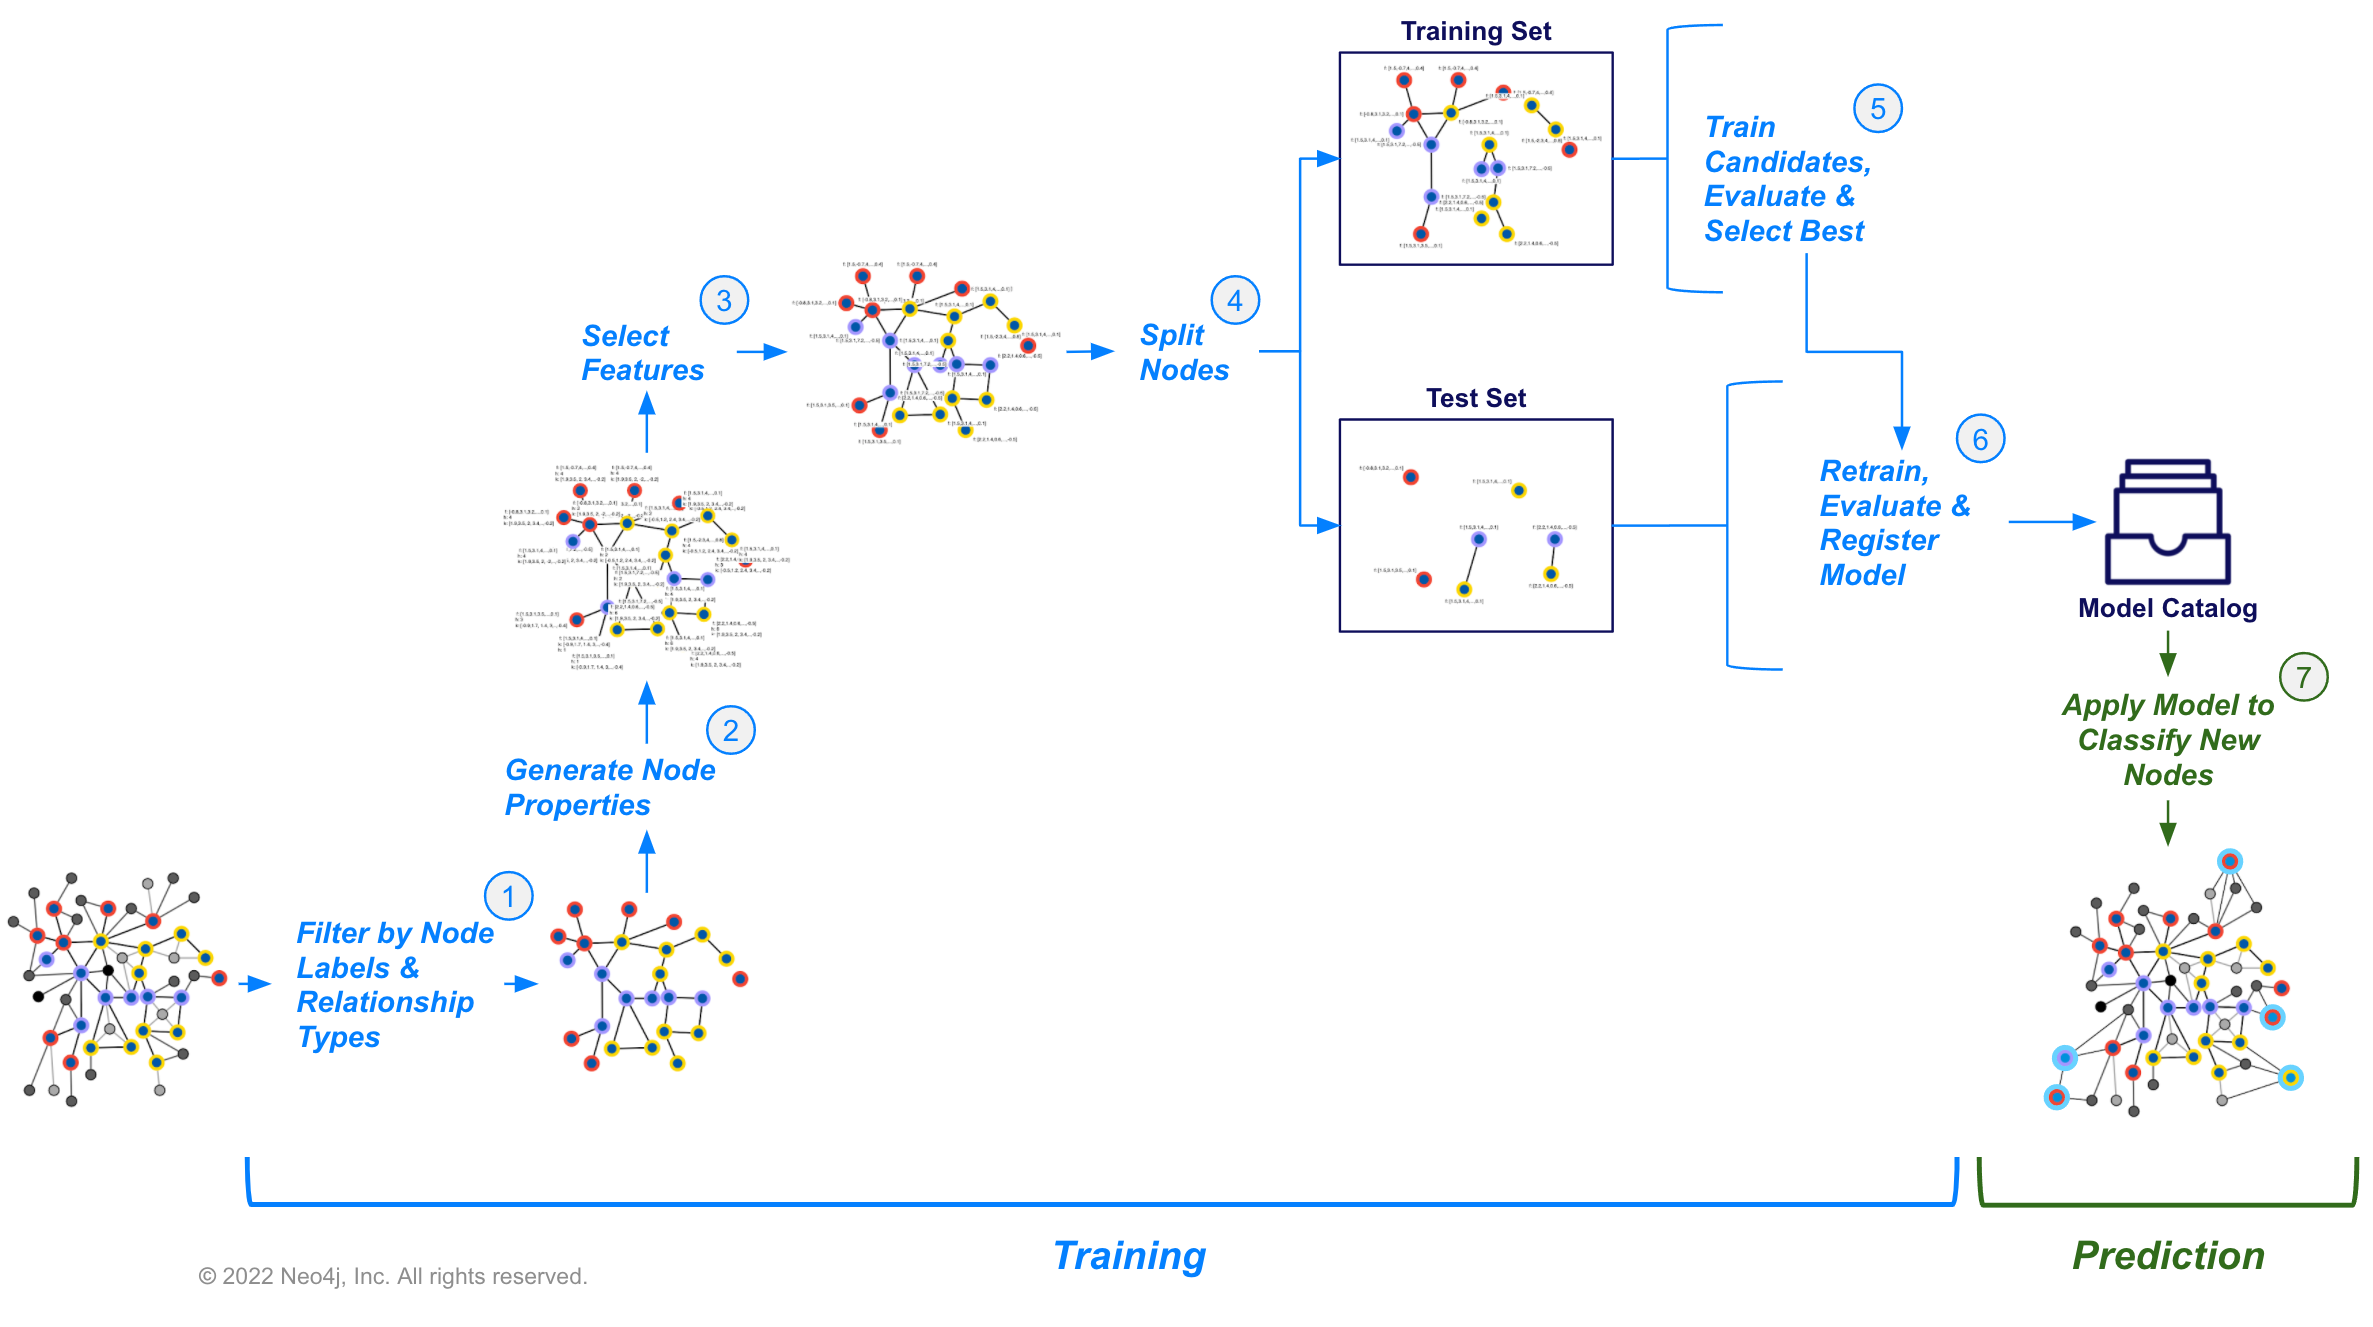
\includegraphics[width=\linewidth,keepaspectratio]{neo4j100}
\end{center}	

\end{frame}

%%%%%%%%%%%%%%%%%%%%%%%%%%%%%%%%%%%%%%%%%%%%%%%%%%%%%%%%%%%%%%%%%%%%%%%%%%%%%%%%%%
\begin{frame}[fragile]\frametitle{Machine Learning: Link Prediction: Problem}

\begin{itemize}
\item Problem: Predicting Actor Relationships with Link Prediction.
\item Domain:  a quick example, we will manufacture a social network out of the graph. We will filter down to just big high grossing movies then create ACTED\_WITH relationships between actors that were in the same movies together
\end{itemize}


\end{frame}

%%%%%%%%%%%%%%%%%%%%%%%%%%%%%%%%%%%%%%%%%%%%%%%%%%%%%%%%%%%%%%%%%%%%%%%%%%%%%%%%%%
\begin{frame}[fragile]\frametitle{Machine Learning: Link Prediction: Problem}



\begin{lstlisting}
//set a node label based on recent release and revenue conditions
MATCH (m:Movie)
WHERE m.year >= 1990 AND m.revenue >= 1000000
SET m:RecentBigMovie;

//native projection with reverse relationships
CALL gds.graph.project('proj',
  ['Actor','RecentBigMovie'],
  {
  	ACTED_IN:{type:'ACTED_IN'},
    HAS_ACTOR:{type:'ACTED_IN', orientation: 'REVERSE'}
  }
);

//collapse path utility for relationship aggregation - no weight property
CALL gds.alpha.collapsePath.mutate('proj',{
    relationshipTypes: ['ACTED_IN', 'HAS_ACTOR'],
    allowSelfLoops: false,
    mutateRelationshipType: 'ACTED_WITH'
});
\end{lstlisting}

\end{frame}
%%%%%%%%%%%%%%%%%%%%%%%%%%%%%%%%%%%%%%%%%%%%%%%%%%%%%%%%%%%%%%%%%%%%%%%%%%%%%%%%%%
\begin{frame}[fragile]\frametitle{Machine Learning: Link Prediction: Problem}

\begin{itemize}
\item This gives us a graph projection with just Actor nodes and ACTED\_WITH relationships, like a 'co-acting' social network. 
\item When we use link prediction in this context, we will be training a model to predict which actors are most likely to be in the same movies together given other ACTED\_WITH relationships already present in the graph. 
\end{itemize}

\begin{lstlisting}
//write relationships back to graph
CALL gds.graph.writeRelationship('proj', 'ACTED_WITH');

//drop duplicates
MATCH (a1:Actor)-[s:ACTED_WITH]->(a2)
WHERE id(a1) < id(a2)
DELETE s;

//clean up extra labels
MATCH (m:RecentBigMovie) REMOVE m:RecentBigMovie;

//project the graph
CALL gds.graph.drop('proj');
CALL gds.graph.project('proj', 'Actor', {ACTED_WITH:{orientation: 'UNDIRECTED'}});
\end{lstlisting}

\end{frame}

%%%%%%%%%%%%%%%%%%%%%%%%%%%%%%%%%%%%%%%%%%%%%%%%%%%%%%%%%%%%%%%%%%%%%%%%%%%%%%%%%%
\begin{frame}[fragile]\frametitle{Machine Learning: Link Prediction: Configure the Pipeline}

\begin{itemize}
\item Create the Pipeline
\item Add Node Properties
\item Add Link Features
\item Configure Relationship Splits
\item Add Model Candidates
\end{itemize}

\begin{lstlisting}
CALL gds.beta.pipeline.linkPrediction.create('pipe');

CALL gds.beta.pipeline.linkPrediction.addNodeProperty('pipe', 'fastRP', {
    mutateProperty: 'embedding',
    embeddingDimension: 128,
    randomSeed: 7474
}) YIELD nodePropertySteps;

CALL gds.beta.pipeline.linkPrediction.addNodeProperty('pipe', 'degree', {
    mutateProperty: 'degree'
}) YIELD nodePropertySteps;
\end{lstlisting}

\end{frame}

%%%%%%%%%%%%%%%%%%%%%%%%%%%%%%%%%%%%%%%%%%%%%%%%%%%%%%%%%%%%%%%%%%%%%%%%%%%%%%%%%%
\begin{frame}[fragile]\frametitle{Machine Learning: Link Prediction: Configure the Pipeline}

\begin{lstlisting}
// configures a symmetric function that takes the properties from the node pair and computes features for the link prediction model. 
CALL gds.beta.pipeline.linkPrediction.addFeature('pipe', 'l2', {
  nodeProperties: ['embedding']
}) YIELD featureSteps;

CALL gds.beta.pipeline.linkPrediction.addFeature('pipe', 'cosine', {
  nodeProperties: ['embedding']
}) YIELD featureSteps;

CALL gds.beta.pipeline.linkPrediction.addFeature('pipe', 'hadamard', {
  nodeProperties: ['degree']
}) YIELD featureSteps;

// configure the relationship splitting which sets the train/test/feature set proportions, the negative sampling ratio, and the number of validations folds used in cross-validation. 
CALL gds.beta.pipeline.linkPrediction.configureSplit('pipe', {
    testFraction: 0.2,
    trainFraction: 0.5,
    negativeSamplingRatio: 2.0
}) YIELD splitConfig;
\end{lstlisting}

\end{frame}

%%%%%%%%%%%%%%%%%%%%%%%%%%%%%%%%%%%%%%%%%%%%%%%%%%%%%%%%%%%%%%%%%%%%%%%%%%%%%%%%%%
\begin{frame}[fragile]\frametitle{Machine Learning: Link Prediction: Configure the Pipeline}

\begin{lstlisting}
// creating model candidates. 
CALL gds.beta.pipeline.linkPrediction.addLogisticRegression('pipe', {
    penalty: 0.001,
    patience: 2
}) YIELD parameterSpace;

CALL gds.beta.pipeline.linkPrediction.addLogisticRegression('pipe', {
    penalty: 1.0,
    patience: 2
}) YIELD parameterSpace;
\end{lstlisting}

\end{frame}

%%%%%%%%%%%%%%%%%%%%%%%%%%%%%%%%%%%%%%%%%%%%%%%%%%%%%%%%%%%%%%%%%%%%%%%%%%%%%%%%%%
\begin{frame}[fragile]\frametitle{Machine Learning: Link Prediction: Train the Pipeline}

\begin{lstlisting}
CALL gds.beta.pipeline.linkPrediction.train('proj', {
    pipeline: 'pipe',
    modelName: 'lp-pipeline-model',
    randomSeed: 7474 //usually a good idea to set a random seed for reproducibility.
}) YIELD modelInfo
RETURN
modelInfo.bestParameters AS winningModel,
modelInfo.metrics.AUCPR.train.avg AS avgTrainScore,
modelInfo.metrics.AUCPR.outerTrain AS outerTrainScore,
modelInfo.metrics.AUCPR.test AS testScore
\end{lstlisting}

\end{frame}

%%%%%%%%%%%%%%%%%%%%%%%%%%%%%%%%%%%%%%%%%%%%%%%%%%%%%%%%%%%%%%%%%%%%%%%%%%%%%%%%%%
\begin{frame}[fragile]\frametitle{Machine Learning: Link Prediction: Prediction with the Model}
This operation supports a mutate execution mode to save the predicted links in the graph projection.


\begin{lstlisting}
CALL gds.beta.pipeline.linkPrediction.predict.stream('proj', {
  modelName: 'lp-pipeline-model',
  sampleRate:0.1,
  topK:1,
  randomSeed: 7474,
  concurrency: 1
})
 YIELD node1, node2, probability
 RETURN gds.util.asNode(node1).name AS actor1, gds.util.asNode(node2).name AS actor2, probability
 ORDER BY probability DESC, actor1
\end{lstlisting}


\end{frame}